\subsection{de.view.overlay.factory}

\rule{\textwidth}{0.4pt} 
\class{OverlayFactory}
public interface OverlayFactory 

\begin{minipage}{0.3\textwidth}
    \begin{figure}[H]
        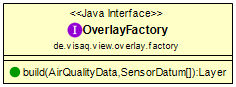
\includegraphics[scale = 0.5
        ]{media/frontend/view/de.view.overlay.factory/OverlayFactory_Class.png}
    \end{figure}
    \end{minipage} \hfill
    \begin{minipage}{0.6\textwidth}
Kapselt die Kontrolle über die Overlay factories
\end{minipage}

Methoden:
\begin{itemize} 
    \item \emph{public Layer build(AirQualityData airquality, SensorDatum[] data)}  Baut einen Overlay mithilfe von der Farbwerte der Luftqualitätsdata und der SensorDaten
\end{itemize}

\rule{\textwidth}{0.4pt} 
\class{InterpolationOverlayFactory}
public class InterpolationOverlayFactory implements OverlayFactory

\begin{minipage}{0.3\textwidth}
    \begin{figure}[H]
        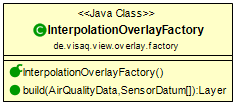
\includegraphics[scale = 0.5]{media/frontend/view/de.view.overlay.factory/InterpolationOverlayFactory_Class.png}
    \end{figure}
    \end{minipage} \hfill
    \begin{minipage}{0.6\textwidth}
Erstellt ein Map Overlay welches die unterschiedlichen Interpolationswerte anzeigt die von unterschiedlichen Sensoren gemessen werden.
\end{minipage}

Methoden:
\begin{itemize} 
    \item \emph{public Layer build(AirQualityData airquality, SensorDatum[] data)}  Baut einen Overlay mithilfe von der Farbwerte der Luftqualitätsdata und der SensorDaten
\end{itemize}

\rule{\textwidth}{0.4pt} 
\class{SensorOverlayFactory}
public class SensorOverlayFactory implements OverlayFactory

\begin{minipage}{0.3\textwidth}
    \begin{figure}[H]
        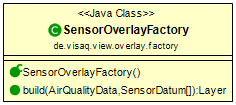
\includegraphics[scale = 0.5]{media/frontend/view/de.view.overlay.factory/SensorOverlayFactory_Class.png}
    \end{figure}
    \end{minipage} \hfill
    \begin{minipage}{0.6\textwidth}
        Erstellt ein Map Overlay welches die unterschiedlichen Sensordata anzeigt die von unterschiedlichen Sensoren gemessen werden.
\end{minipage}

Methoden:
\begin{itemize} 
    \item \emph{public Layer build(AirQualityData airquality, SensorDatum[] data)}  Baut einen Overlay mithilfe von der Farbwerte der Luftqualitätsdata und der SensorDaten
\end{itemize}

\rule{\textwidth}{0.4pt} 
\class{OverlayBuilder}
public class OverlayBuilder

\begin{minipage}{0.5\textwidth}
    \begin{figure}[H]
        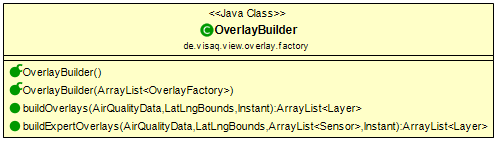
\includegraphics[scale = 0.5]{media/frontend/view/de.view.overlay.factory/OverlayBuilder_Class.png}
    \end{figure}
    \end{minipage} \hfill
    \begin{minipage}{0.4\textwidth}
Schnittstelle füt die Overlay factory. Hier werden die Overlays mithilfe von speziellen factories für die Karten gebaut
\end{minipage}

Methoden:
\begin{itemize} 
    \item \emph{public OverlayBuilder()} Standard Builder, welcher Overlay Factory und Interpolation Overlay Factory verwendet.
    \item \emph{public OverlayBuilder(ArrayList<OverlayFactory> factories)} Builder für das bauen von Overlays mithilfe von factories.
    \item \emph{public ArrayList<Layer> buildOverlays(AirQualityData airquality, LatLngBounds latLngBounds, Instant time)} Erstellt eine ArrayList mit den unterschiedlichen Layern anhand der ausgewählten Luftqualitätsdata, der gewählten Zeit und den Bounds.
    \item \emph{public ArrayList<Layer> buildExpertOverlays(AirQualityData airQuality, LatLngBounds latLngBounds, ArrayList<Sensor> selectedSensortypes, Instant time)}  Erstellt eine ArrayList mit den unterschiedlichen Layern anhand der ausgewählten Luftqualitätsdata, der gewählten Zeit, der gewählten Sensortypen und den Bounds.
\end{itemize}